\documentclass[10pt,a4paper]{article}
\usepackage[margin=22mm,headheight=15pt]{geometry}
\usepackage[T1]{fontenc}
\usepackage{lmodern,microtype,amsmath,amssymb,booktabs,array,longtable,graphicx,xcolor,tikz,fancyhdr}
\usepackage[hyphens]{url}
\usepackage[numbers,sort&compress]{natbib}
\usepackage[colorlinks=true,linkcolor=teal,citecolor=teal,urlcolor=teal]{hyperref}
\usetikzlibrary{arrows.meta,positioning,fit}
\definecolor{ink}{HTML}{142236}
\definecolor{teal}{HTML}{168C85}
\definecolor{violet}{HTML}{7863CE}
\definecolor{pale}{HTML}{F0F4F8}
\hypersetup{pdftitle={AGI ALPHA: Constructing the Productive Arrangement},pdfauthor={MONTREAL.AI},pdfsubject={Executed synthetic dispatch and conditional native-account economics}}
\pagestyle{fancy}
\fancyhf{}
\fancyhead[L]{\small\textsf{MONTREAL.AI / TRANSFORMATIONAL 063}}
\fancyhead[R]{\small\textsf{RESEARCH EDITION}}
\fancyfoot[L]{\footnotesize Executed software. Synthetic profiles. Simulated commerce.}
\fancyfoot[R]{\thepage}
\setlength{\parindent}{0pt}
\setlength{\parskip}{5pt}
\setlength{\emergencystretch}{2em}
\setlength{\tabcolsep}{5pt}
\renewcommand{\arraystretch}{1.2}
\newcommand{\code}[1]{\texttt{\small #1}}
\newcommand{\state}[1]{\textsf{\textbf{#1}}}
\newcommand{\NativeAbstract}{The primary four-period native simulation records four accepted settlements, US\$250 revenue, US\$155.80 operating expense, US\$23.55 modeled tax and US\$70.65 net profit; copycat and no-purchase scenarios each lose US\$128.}
\newcommand{\NativeResults}{\textbf{Source-matched operating result.} Four separate accounts each start with US\$100,000; the central account is the primary challenge and returns are never pooled. All four key-free native replays pass. This is a development operation, not a claim that the final committed source has already completed release qualification.
\begin{center}\small
\begin{tabular}{lrrl}\toprule
Authored scenario & Accepted & Net profit (US\$) & Commercial decision\\\midrule
Central & 4 & 70.65 & Conditional GO\\
Copycat undercuts & 0 & -128.00 & Not established\\
Buyer declines & 0 & -128.00 & Not established\\
Supplier failure / 4x cost & 3 & 2.40 & Not established\\\bottomrule
\end{tabular}\end{center}
Central recognized and collected planning revenue is US\$250; operating expense is US\$155.80 and the authored 25\% positive-income tax provision is US\$23.55, giving total incurred and paid expense of US\$179.35. Closing cash is US\$100,070.65, with US\$4 tail reserve, no unpaid liability and US\$100,066.65 available. The tax envelope is a simulation assumption, not an actual tax bill. A US\$15 instrument investment is recorded as EARNED-funded. Its forecast US\$20 benefit is an authored hypothesis, not a realized gain. The supplier case fails the registered three-core-cycle criterion: two accepted core cycles against three required, despite positive period profit. The two zero-sale arms retain US\$128 of development, acquisition and maintenance expense.}
\newcommand{\RegressionResults}{The numerical native-account controls include a US\$270 profitable tie, a US\$730 complete-cost loss despite a technical win, a specialist with US\$50 negative incremental value, US\$99,990 cash with a US\$10 loss, and US\$270 current profit with US\$730 development unrecovered. Another case retains US\$50 payable after US\$100,050 incurred expense; a failed delivery retains US\$7 expense after refund. The implemented accounting policy expenses development immediately and refuses a duplicate capitalized-plus-expense policy. A full capitalized-asset/amortization reporting variant is not implemented and is an explicit remaining mandatory case; this edition does not claim that variant passed. The exact test command and source-matched execution receipt establish regression status separately from this table.}
\newcommand{\SuccessorResults}{The native retained-asset arm incurs US\$18 of declared complete successor cost including the US\$15 instrument, versus US\$3 for the ordinary route; each accepts one fresh result. The observed incremental cost is therefore US\$15 with no additional accepted work. The ex-ante conditional investment case does not survive as realized retention advantage. Continue the profitable base offering while declining further unsupported specialist retention.}
\newcommand{\FinalVerdict}{The central account passes conditional commercial criteria, while copycat competition and buyer refusal defeat profitability. Blue Sky and retained successor advantage remain unestablished, and the optional asset loses its matched economic comparison.}
\newcommand{\NativeReproduction}{Run from the repository root:
\begin{quote}\small\ttfamily
python3 -m connected\_enterprise.transformational063 run --output /absolute/new/native\\
python3 -m connected\_enterprise.transformational063 audit --output /absolute/new/native
\end{quote}
The retained key-free operation is under the campaign's \code{native/} directory, including frozen source, all four public exports, protocol, source manifest, report and audit. Audit it with its own frozen source. Its source identity begins \code{b962739069069f700}; the full SHA256 is recorded in the report. Private recovery files are excluded.}

\begin{document}
\thispagestyle{empty}
{\color{teal}\large\textsf{AGI ALPHA FLYWHEEL}}\hfill{\textsf{1 NOVEMBER 2026}}
\vspace{11mm}

{\color{ink}\fontsize{31}{34}\selectfont\textbf{Constructing the\\productive arrangement}}

\vspace{4mm}
{\Large Transformational intelligence as an executable question}

\vspace{6mm}
{\large MONTREAL.AI}\par
{\normalsize Research and engineering edition 063}

\vspace{8mm}
\colorbox{pale}{\parbox{.94\linewidth}{\vspace{3mm}\textbf{The experiment.} Can a complete arrangement make useful work attainable, deliver a checkable result, sustain its full simulated costs, and leave a successor better equipped? The unit of progress is an accepted outcome together with the means and financing that make it achievable.\vspace{3mm}}}

\vspace{5mm}
\textbf{Abstract.} We construct a bounded dispatch-planning offering that pools small flexible loads under a fixed aggregate contract, preserves participant energy requirements, assigns compensation above declared displacement costs, and emits an independently replayable schedule. Four frozen synthetic requests test three successive one-event quantities and a fresh two-event successor. Each isolated-resource arm is infeasible; pooled production and an unrestricted conventional mixed-integer optimizer both pass all four requests with identical artifacts and compensation. An independently delegated generalist also constructs an accepted successor from the request alone. The structural change matters relative to isolated service, while algorithmic superiority and inherited technical advantage are not established. The same deliverable is connected to the existing journaled enterprise account, with native acceptance, settlement, obligations and funding attribution. Separate decisions and numerical regressions prevent technical quality, accounting profit, available cash, project payback and investment source from substituting for one another. \NativeAbstract{} The contribution is an inspectable complete software arrangement and a conservative decision boundary. It is not physical demand response, observed customer demand, a newly discovered industry, a complete-cost frontier-model comparison, or the US\$3 billion trailing-year profit objective.

\vfill
{\color{ink}\large\textbf{Build the means. Deliver the outcome. Test what comes next.}}\par
\small Source, acceptance contracts, controls and negative findings remain part of the result.
\newpage

\section{Purpose, construction and the frontier}
An improved answer and an expanded productive possibility are different achievements. Let $K$ be the admitted stock of productive means, $b$ a complete resource budget, and $u$ a beneficiary outcome with an unchanged acceptance contract. Following the capability-frontier framing in Out-Evolve~\cite{outevolve2026}, define
\begin{equation}
\mathcal F_b(K)=\{u:\text{an authorized use of }K\text{ delivers accepted }u\text{ within }b\}.
\end{equation}
A construction may enlarge this set, lower the cost of existing members, reveal a useful question, or fail. Its full comparison charges construction, checking, failures, maintenance and transfer. An unrestricted conventional route can already possess the same means. A difference relative to a restricted baseline must not be promoted into a universal advantage.

Transformational Intelligence~\cite{ti2026} separates the intended purpose, problem formulation and evaluator. Its exact causal example changes an information restriction, but an unrestricted optimal planner matches the constructed intervention policy. Invent the Economy~\cite{economy2026} treats the capability, participant benefit, payment arrangement and cash sequence jointly; positive expected contribution need not finance construction. We use these distinctions operationally: change a removable service boundary while keeping required delivery, participant interests and cash authority fixed.

\subsection{A consequential direction with a small decisive test}
Small flexible resources can have useful aggregate value while each is individually below a service threshold. The first product here is a \emph{dispatch-planning artifact}: a schedule and compensation allocation that another program can check. Physical resource response is outside this experiment. Aggregation itself is established practice. FERC describes pooling to meet size and performance requirements, together with location, metering, telemetry and coordination conditions~\cite{ferc2222}; quantitative aggregation and disaggregation have a substantial technical precedent~\cite{mueller2017}. The strongest ordinary complete route is therefore an essential control, not an optional challenge.

\subsection{Three different possibilities before commitment}
\begin{tabular}{p{.23\linewidth}p{.34\linewidth}p{.35\linewidth}}
\toprule
Possibility & Missing means to investigate & Bounded probe and decision \\
\midrule
Pooled flexibility & Verifiable joint schedule, participant outside options and funded delivery & Execute fixed integer-energy contracts; selected for local construction, not novel aggregation.\\
Retrospective measurement & Evidence that identifies a useful past state & A two-unknown, one-observation indistinguishable pair blocks the toy inverse contract. New observation needed.\\
Complementary manufacturing & Compatible routes and accepted physical interfaces & A finite process-set join is feasible, but tolerance, traceability, machine access and price evidence are absent.\\
\bottomrule
\end{tabular}

The latter two probes are prerequisite checks, not full domain evaluations. They do not establish that all historical sensing is impossible or that a manufacturing venture is qualified. The seven-question admission record preserves this limit and separates selecting a test from issuing Blue Sky Flagship GO.
\newpage

\section{The executable kernel and unchanged acceptance}
There are four devices and four one-hour slots. Device $i$ has baseline energy $b_{it}$, available slot limit $p_{it}$ and required total energy $E_i$. The constructed dispatch $x_{it}$ and event reductions $r_{it}$ satisfy
\begin{align}
0\leq x_{it}&\leq p_{it}a_{it}, & \sum_t x_{it}&=E_i,\\
r_{it}&=b_{it}-x_{it}\geq0 &&\text{for event slots},\\
\left\lfloor(1-\delta)\sum_i r_{it}\right\rfloor&\geq q_t. &&
\end{align}
All energy is integer Wh. The derating allowance is $\delta=0.05$. An active device receives its declared linear displacement cost plus a positive fixed margin:
\begin{equation}
m_i=c_i\sum_{t\in\mathcal E}r_{it}+\eta\,\mathbf 1\left[\sum_{t\in\mathcal E}r_{it}>0\right],\qquad \sum_i m_i\leq B.
\end{equation}
Here $B$ is the authored buyer's resource-compensation budget; it is not enterprise revenue. Every device retains 80,000 Wh across the horizon, with 40,000 Wh slot limits and baseline $(40{,}000,40{,}000,0,0)$. A participant receives a US\$1 modeled margin when active. These are authored synthetic profiles, not measured electrical loads or revealed preferences.

The production method is the established HiGHS mixed-integer optimizer through SciPy. Both the AGI ALPHA and ordinary complete controls may use it. The checker independently replays request identity, integer energy, resource limits, aggregate delivery, compensation and budget. It does not trust a producer success flag. Shared host and agent-family custody remain a limitation of independence.

\begin{figure}[h]
\centering
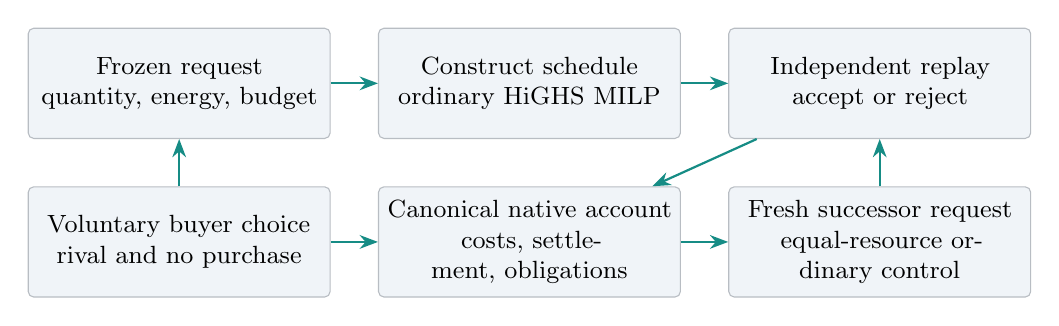
\begin{tikzpicture}[node distance=6mm,box/.style={draw=ink!30,rounded corners=2pt,fill=pale,text width=36mm,minimum height=14mm,align=center,font=\small},arr/.style={-{Stealth},thick,teal}]
\node[box] (need) {Frozen request\\quantity, energy, budget};
\node[box,right=of need] (produce) {Construct schedule\\ordinary HiGHS MILP};
\node[box,right=of produce] (check) {Independent replay\\accept or reject};
\node[box,below=of need] (choice) {Voluntary buyer choice\\rival and no purchase};
\node[box,below=of produce] (account) {Canonical native account\\costs, settlement, obligations};
\node[box,below=of check] (next) {Fresh successor request\\equal-resource ordinary control};
\draw[arr] (need)--(produce);\draw[arr] (produce)--(check);
\draw[arr] (choice)--(account);\draw[arr] (check)--(account);\draw[arr] (account)--(next);
\draw[arr] (choice)--(need);\draw[arr] (next)--(check);
\end{tikzpicture}
\caption{One causal enterprise, with separate acceptance and finance. Physical dispatch and external customers are not represented as observed results. The successor inherits a usable interface, not automatic proof or spending authority.}
\end{figure}

The paid offering directly exercises this kernel. An accepted schedule can support a planning-service settlement under the simulated contract; a hypothetical grid benefit cannot. This boundary prevents modeled resource compensation or avoided physical cost from being misrecognized as collected enterprise revenue.
\newpage

\section{Executed technical comparison}
The registration freezes single-event targets of 100, 110 and 120 kWh and a fresh two-event target of 65 kWh in each of the first two slots. Under 5\% derating, a single 40 kWh resource cannot satisfy any request. All four requests have a feasible pooled solution.

The retained technical record is an engineering re-execution after sparse-constraint and numerical-safety corrections, with unchanged profiles, policy and acceptance. It is not an untouched confirmation set, and no favorable request or seed was substituted.

{\small\setlength{\tabcolsep}{3pt}
\begin{tabular}{lrrrr}
\toprule
Request & Isolated accepted & Ordinary accepted & Pooled accepted & Compensation (US\$)\\
\midrule
100 kWh event & 0 & 1 & 1 & 18.052800\\
110 kWh event & 0 & 1 & 1 & 20.158000\\
120 kWh event & 0 & 1 & 1 & 23.579000\\
65 + 65 kWh successor & 0 & 1 & 1 & 18.526600\\
\midrule
Total accepted / attempted & 0/4 & 4/4 & 4/4 & Not additive enterprise value\\
\bottomrule
\end{tabular}
}

\begin{figure}[h]
\centering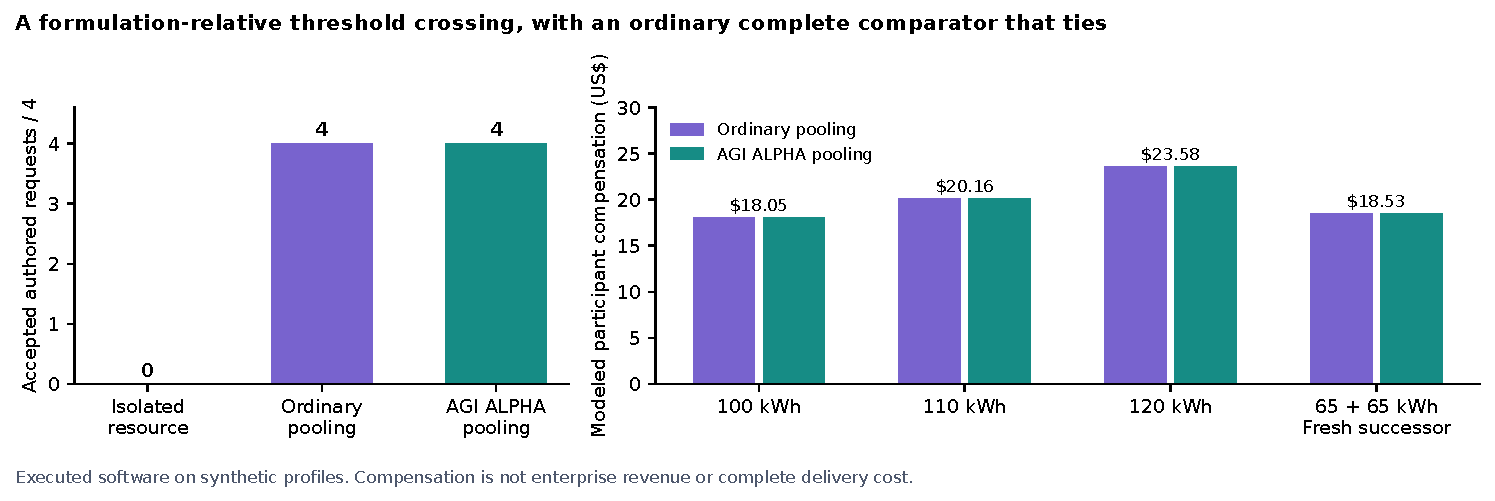
\includegraphics[width=\linewidth]{technical-results.pdf}
\caption{Actual software execution on authored profiles. Ordinary and pooled production have identical accepted artifacts and participant compensation in every case. The cost of compensating resources is distinct from the complete cost of delivering a planning product.}
\end{figure}

\textbf{What changed.} Allowing a coalition changes the attainable outcome relative to isolated resources. The quantity requirement, energy conservation and compensation checks remain fixed. This is an explicit formulation-relative effect.

\textbf{What did not improve.} The unrestricted ordinary method constructs the same result. The technical comparison does not establish algorithmic superiority, a proprietary discovery, an AI advantage or an industry that previously could not exist. Timing telemetry is retained per command; a single microbenchmark is not a stable cost advantage.

\textbf{Direct included generalist.} A separately delegated included agent received only the fresh successor request, without the repository kernel. It constructed an independent SciPy/HiGHS program whose artifact passed the precommitted integer checker: 65 + 65 kWh, with US\$18.526600 compensation, tying the construction. The recorded solver process used 2.6357 seconds wall and 4.4474 seconds CPU. Those figures exclude agent construction and inference; complete billing remains unknown. This is a scoped technical control, not evidence of full-cost or vendor-wide superiority. No separately billable API was used.

\textbf{Human-market benchmark.} No sourced quote for the same accepted planning scope was collected. We do not invent human task-hours or transform compensation into a consulting rate. $H$, the price of a truly equivalent human-delivered service, remains unknown; $H-C$ is not reported as revenue. A later commercial study must obtain a scope-matched professional price or a supported avoided-cost alternative.
\newpage

\section{Strategic commerce and the financial constitution}
The commercial path keeps the existing \code{JournalAccount} and mandatory adaptive \code{Account}. Buyer budgets, rival alternatives, supplier conditions, refusal, failed work and settlement terms are explicit simulated inputs. Production artifacts are executed. A sale is not inferred from a useful schedule. The native ledger recognizes contract revenue and obligations; the decision view reads its exported evidence rather than maintaining another balance.

The experiment uses finite authored choice/quote scenarios with public information, rather than a validated equilibrium or a learned population of autonomous competitors. Any policy conclusion is conditional on these scenarios and the permitted observations.

\NativeResults{}

Four independent financial questions prevent misleading conclusions:
\begin{align}
\Pi &= R_{\rm earned}+R_{\rm recovery}-C_{\rm incurred},\\
\operatorname{Cash}_{t+1}&=\operatorname{Cash}_t+\operatorname{Collections}_t+\operatorname{Financing}_t-\operatorname{Payments}_t-\operatorname{Capex}_t,\\
\operatorname{Available}_t&=\operatorname{Cash}_t-\operatorname{Obligations}_t-\operatorname{Reserves}_t-\operatorname{Commitments}_t.
\end{align}
Project payback separately asks how much original construction/investment outlay remains unrecovered by attributable project cash returns. Positive period profit can coexist with incomplete payback. Available opening equity can fund an affordable investment without being earned profit. Funding attribution records that difference.

\begin{center}
\begin{tabular}{p{.23\linewidth}p{.68\linewidth}}
\toprule
State & Meaning and counterexample\\
\midrule
Accounting profit & Earned revenue minus incurred costs. An unpaid expense remains a cost and liability.\\
Project payback & Recovery of original outlays. A profitable period need not recover construction already paid.\\
Available cash & Cash after protected obligations and commitments. Deposits and borrowing can create cash without profit.\\
Investment source & Unrestricted earned cash, opening equity, debt or declared mixture. Affordability alone does not prove earned-profit funding.\\
\bottomrule
\end{tabular}
\end{center}

Complete AI-native costs include development/search, unsuccessful attempts, production, verification, infrastructure, acquisition, support, maintenance, refunds, financing and residual obligations as applicable. No fictional human salaries are introduced. Modeled envelopes remain conditional; actual unmeasured model/host billing stays unknown. A future capitalization view must charge construction cash once and distinguish later amortization; the implemented policy expenses development immediately.
\newpage

\section{Independent decisions and numerical regression controls}
Commercial GO asks for repeatable positive complete-cost simulated economics with viable obligations. Blue Sky Flagship GO asks for a consequential enabling effect against the appropriate complete route. Investment GO asks for affordable positive incremental benefit under a declared objective. Successor GO asks whether fresh inherited use adds accepted value or useful feasibility under matched resources. These decisions cannot be replaced by a single all-purpose success flag.

\begin{longtable}{p{.39\linewidth}p{.53\linewidth}}
\toprule
Numerical regression condition & Required decision invariant\\
\midrule
\endhead
Conventional method ties or wins, business profitable & Commercial decision may pass; no technical superiority claim.\\
Technically impressive, complete-cost loss & Preserve technical result; reject commercial profitability.\\
Profitable base, specialist costs exceed incremental benefit & Continue base; hold optional retention/investment.\\
Positive cash, negative accounting profit & No profitability claim from seed, debt or timing.\\
Positive period profit, incomplete project payback & Report payback gap; permit justified affordable investment with actual source.\\
Incurred expense cannot yet be paid & Preserve expense and payable; no disappearing liability.\\
Capitalized development followed by amortization & One cash construction payment; consistent accounting expense timing.\\
Opening-equity or debt-funded investment & No earned-profit-funded characterization.\\
Failed acceptance after resource use, then refund & Costs remain; refund and revenue treatment reconcile.\\
Inherited capability works but adds no economic value & No retention advantage; base operation may remain viable.\\
\bottomrule
\end{longtable}

\RegressionResults{}

These tests establish implementation invariants within declared financial treatments. They are not commercial observations and cannot calibrate willingness to pay. A precision error in a stop rule can otherwise reject good ordinary commerce because a specialist loses, or approve a losing enterprise because opening cash is large. Every material HOLD/STOP therefore needs its own comparator, metric, threshold, numerical outcome and evidence.

The primary objective remains a US\$100,000 initial simulated account and US\$3 billion complete-cost profit over a trailing 365-day operating window at its registered endpoint. Revenue, valuation, cash, total multiyear profit and annualized short cohorts are ineligible substitutes. This edition does not demonstrate that milestone.
\newpage

\section{Successor and what has become possible}
The fresh successor has two 65 kWh events rather than the predecessor's single event. The retained request, production and checking interface handles the new contract. Its schedule passes the same acceptance semantics, and each resource retains its required energy. That is a useful new request handled by an installed interface.

The equal-resource control is free to rebuild or invoke the same ordinary mixed-integer method. It also passes. Both pay US\$18.526600 in modeled participant compensation, for an observed difference of US\$0. There is no evidence that the inherited method expands the frontier beyond this strong ordinary route. A later-in-time accepted result is not automatically causally enabled by the predecessor. Retention could still be operationally useful, but its construction, maintenance, validation and transfer costs must be justified by fresh incremental returns.

\SuccessorResults{}

\subsection{Why-now evidence and its limits}
The 26 October public computer-use release motivates testing lower-cost workflow construction and maintenance~\cite{terra2026}; its vendor prices are not measured cost per accepted dispatch. The same week's scientific release exposes artifacts for examination while explicitly distinguishing raw generated material from scientific understanding~\cite{science2026}. The public correction/withdrawal history~\cite{mathhistory2026} reinforces binding the actual statement and dependencies rather than trusting a formalization label. Risk-proportionate VVUQ~\cite{nist2026} is relevant to any future physical extension. None of these announcements makes this small deterministic experiment a scientific discovery engine.

\subsection{The next decisive evidence}
A stronger claim requires measured device behavior and uncertainty, permissioned telemetry/control, a specific market's applicable qualification and anti-double-counting rules, scope-matched rival prices, observed buyer decisions, complete lifecycle costs and repeated funded operations. A successor advantage additionally needs fresh work and an equally resourced ordinary route that may build its own means. These are substantive missing observations, not cosmetic readiness items.

\textbf{Scientific verdict.} This edition constructs and checks a complete digital arrangement. It demonstrates a threshold effect relative to isolated resources and preserves conventional and generalist ties. \FinalVerdict{} Physical transformation, a new industry, general autonomous invention, direct-model superiority and civilization-scale consequences are not established. The broader ambition remains to make valuable outcomes sustainably attainable by changing their productive prerequisites; the evidence here remains the specific software, comparisons and simulated accounts actually executed.
\newpage

\section{Reproducibility and evidence custody}
The executable registration is \code{flexibility063/REGISTRATION.json}; requests are \code{flexibility063/profiles.json}. The technical experiment is:
\begin{quote}\small\ttfamily
python3 -m flexibility063.experiment --output /absolute/new/technical
\end{quote}
The retained technical result is \code{campaign/transformational-063/TECHNICAL.json}. Its exact registration, profile, production-source, request and artifact SHA256 values bind each comparison. The command logs retain measured CPU/wall telemetry without treating unknown billing as zero.

The request-only generalist control is under the campaign's \code{direct-generalist/} directory: independent source, request, dispatch, process receipt, acceptance and scope. Its accepted artifact SHA256 equals the successor artifact recorded by the technical experiment. Full agent construction/inference consumption is unmetered.

\NativeReproduction{}

Financial recovery authority stays private. A key-free export supports read-only audit, not resuming the original business. Source updates require their own qualification; a paper build cannot turn an earlier run into a final source-matched release. The Markdown report identifies the evidence scope, command receipts and exact qualification status at publication. No failed financial state is erased to improve a headline.

\textbf{Build the paper.} From this directory, regenerate the technical figure with \code{make\_figures.py}, then run \code{pdflatex paper.tex}, \code{bibtex paper}, and \code{pdflatex} twice. The bibliography includes pinned foundation URLs. The source-provenance JSON gives downloaded PDF hashes; the source-review Markdown records inspected content and interpretation limits. Visual QA renders the compiled pages and checks legibility and page boundaries.

\begingroup
\footnotesize
\setlength{\bibsep}{3pt}
\bibliographystyle{plainnat}
\bibliography{references}
\endgroup
\end{document}
